\chapter{Wheatstone Bridge} \labchap{wheatstone_bridge}
The Wheatstone Bridge is a configuration of four resistors in two voltage dividers, as shown in Figure \ref{fig:wheatstone_bridge}, that is sensitive to minute changes in resistance.
Resistors $R_1$ and $R_2$ form the first divider and $R_3$ and $R_4$ form the second divider.
The bridge has at least three different solutions, depending on the configuration and desired application.
For applications where $R_1$, $R_2$, and $R_3$ are known to a high precision, then $R_4$ can be determined to an equally high precision by adjusting $R_3$ until the voltage potential between points $B$ and $D$ is near 0, i.e. the bridge is ``balanced''.
However, for most embedded applications, $R_4$ cannot be determined by balancing the bridge, so either the general solution or linearization must be used.
For simplicity, only the linearization solution will be examined here.

\begin{figure}[h!]
    \caption{A generalized wheatstone bridge}
    \labfig{wheatstone_bridge}
    \centering
    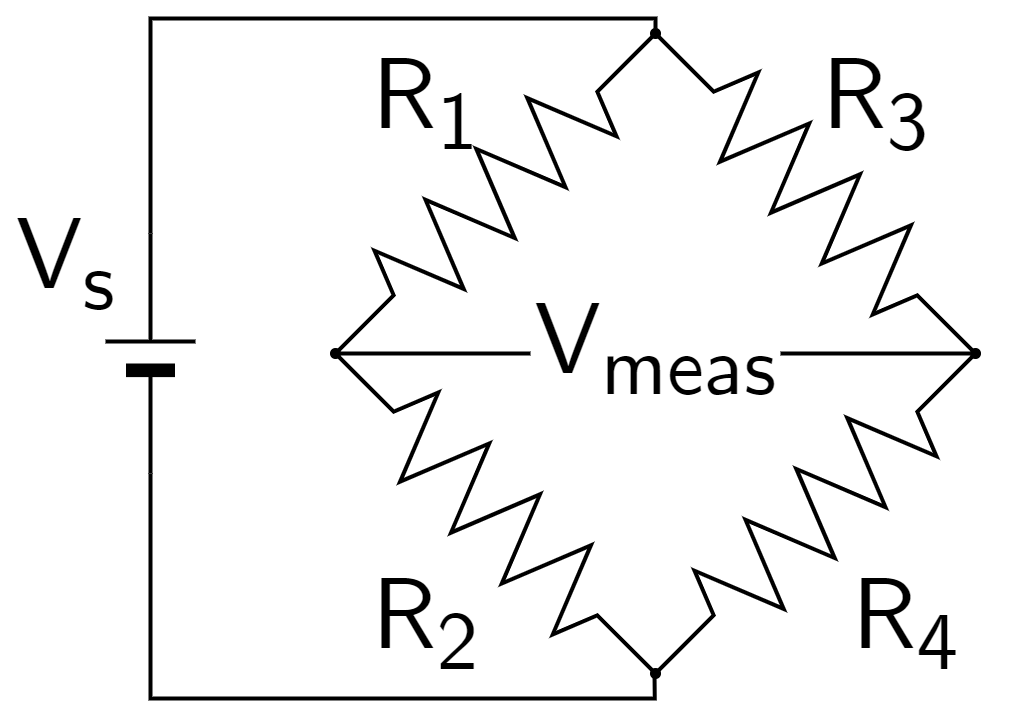
\includegraphics[height=1.5in]{appendices/wheatstone_bridge/wheatstone_bridge.png}
\end{figure}

For the linear solution, the circuit adds an operational amplifier between points $D$ and $B$ and assumes that $R_1=R_2=R_3=R_0$ and $R_4 = R_0 + \Delta R$ and the op-amp is an ideal component ($R_{\text{amp}}$ = 0).
Because of this, the voltage potential at Point $B$ will have a constant value of:

\begin{equation*}
    V_B = \frac{R_0 V_s}{R_0 + R_0} = \frac{V_s}{2}
\end{equation*}

\begin{figure}[h!]
    \caption{A linearized wheatstone bridge}
    \labfig{wheatstone_bridge_linearized}
    \centering
    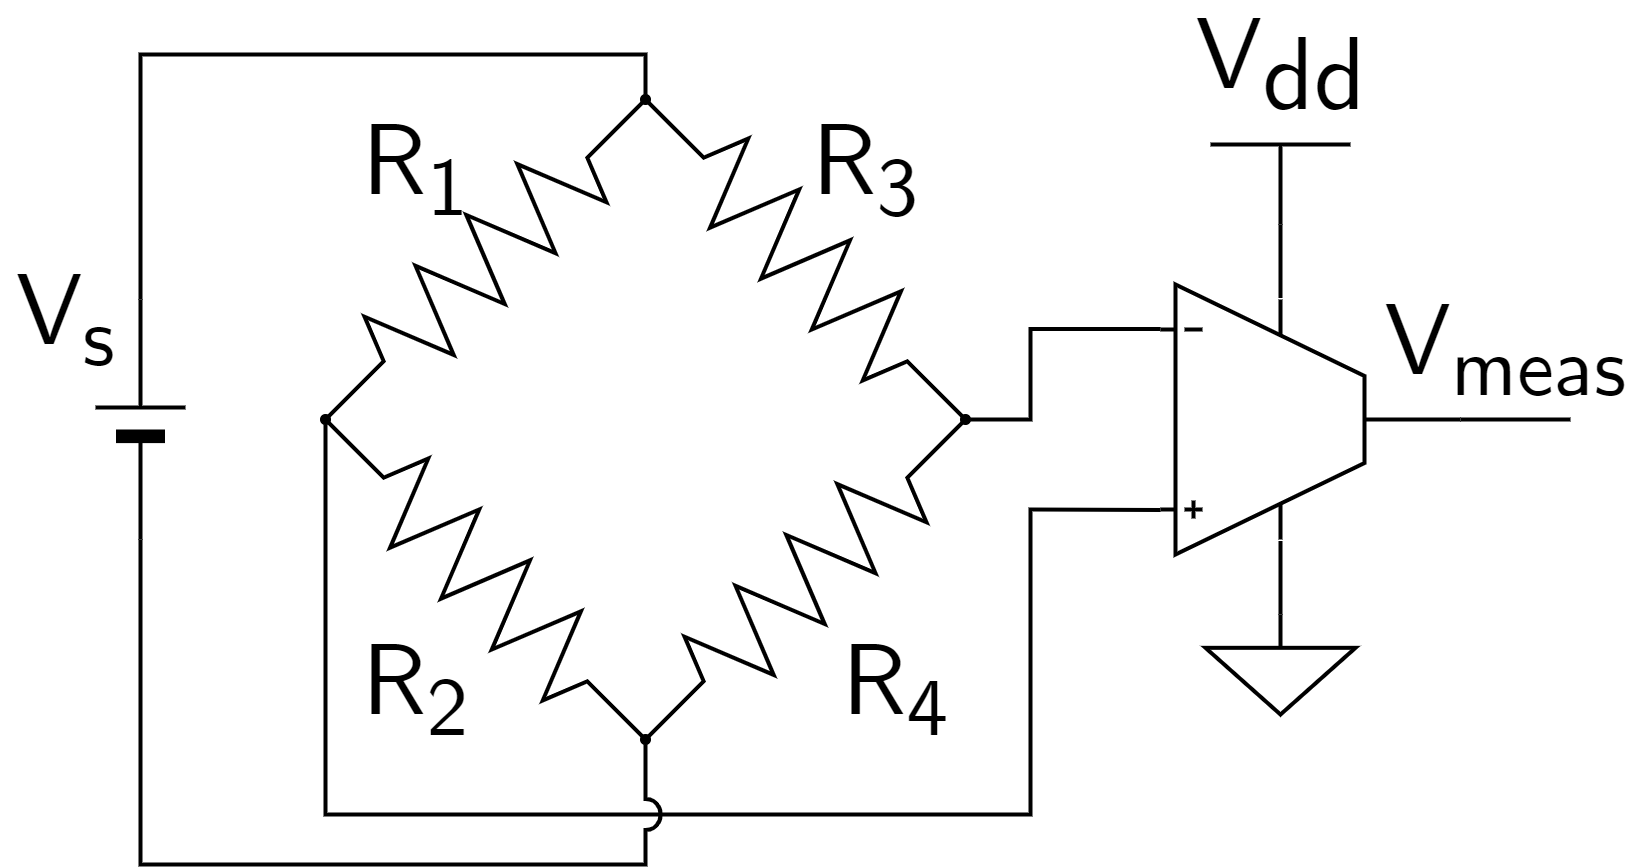
\includegraphics[height=1.5in]{appendices/wheatstone_bridge/wheatstone_bridge_linearized.png}
\end{figure}

Likewise, the op-amp will force the voltage at Point $D$ to have the same voltage as $B$ such that, $V_D = V_B = \frac{V_s}{2} $.
This forces a constant current of $\frac{V_s}{2R_0} $ through $R_3$ and into the sensor.
By Ohm's law, the voltage across the sensor will therefore be:

\begin{align*}
    V_4 &= \frac{V_s}{2R_0} \cdot R_0(1+\Delta R) \\
        &= \frac{V_s}{2} + \frac{V_s}{2} \Delta R
\end{align*}

By applying Kirchoff's voltage law, the potential between the amplifier output and ground, $V_{out} $, is:

\begin{align*}
    V_{\text{meas}} &= -V_4 + V_D \\
            &= -\left( \frac{V_s}{2} + \frac{V_s}{2} \Delta R\right) + V_D \\
    V_{\text{meas}} &= -\frac{V_s}{2} \Delta R
\end{align*}

The measured output voltage now linearly changes with the resistive sensor irregardless of if the sensor changes linearly itself.
If the manufacturer of the sensor provides a table or equation that relates the sensor resistance to a real-world value, we can find the sensor resistance via:

\begin{align*}
    R_4 &= R_0 + \Delta R \\
        &= R_0 - \frac{2V_{out}}{V_s}
\end{align*}